 \chapter{对称性与点群}\label{ch:b3:point-groups}

将雪花转过六十度，图样不变；将苯分子转过同样的角度，
其六个碳原子和六个氢原子恰好各自落到原来的位置上。
分子的对称性在计算之前就决定了它的若干性质：
能否具有偶极矩，能否以两种互为镜像的形式存在，
其中哪些振动能吸收红外线，哪些轨道可以混合。
为了运用对称性，化学家借用了数学中的群论语言。
本章定义分子的对称操作，
将它们归入分子的点群，
给出求点群的步骤，证明关于极性与手性的两个定理，
并引入
\cref{ch:b3:group-theory-applied}所依托的特征标表。

\begin{recall}
本科一年级分册用价层电子对互斥模型预测分子形状，
定义了极性分子的偶极矩，并定义了手性：手性分子
不能与其镜像叠合。本科二年级分册用文字方式运用对称性，
构造了\ce{H2O}和\ce{NH3}的片段轨道。
\end{recall}

\begin{omfigure}
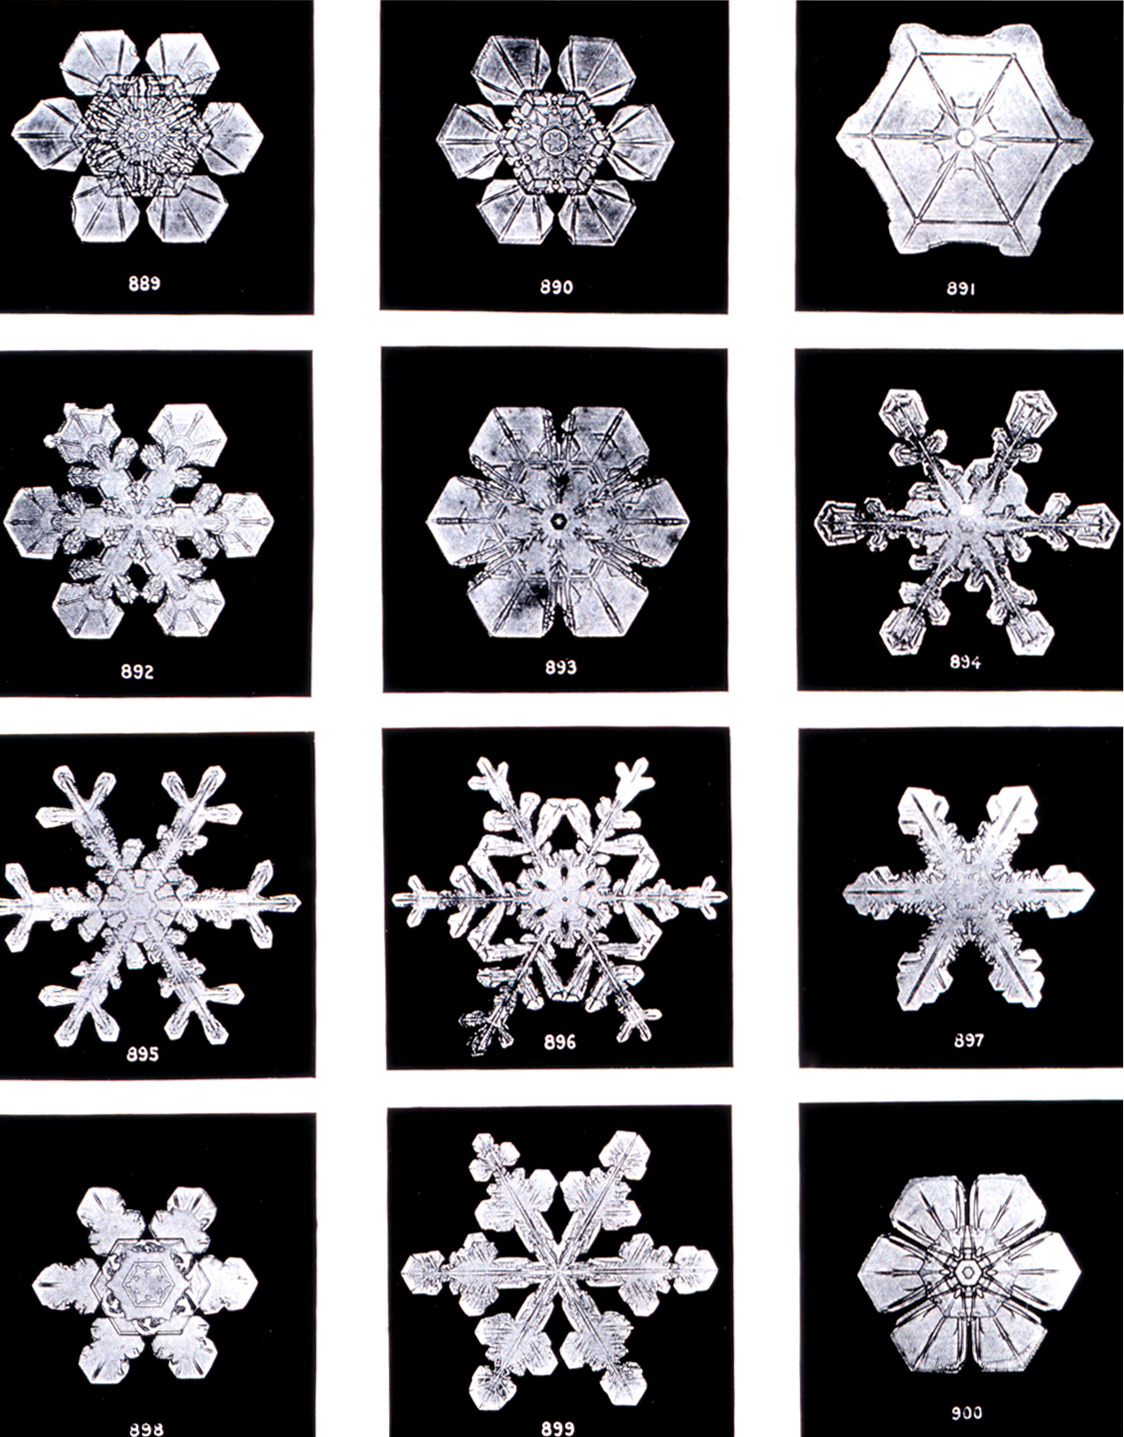
\includegraphics[width=0.4\linewidth]{images/book4/bentley-snowflakes.jpg}\hspace{1em}%
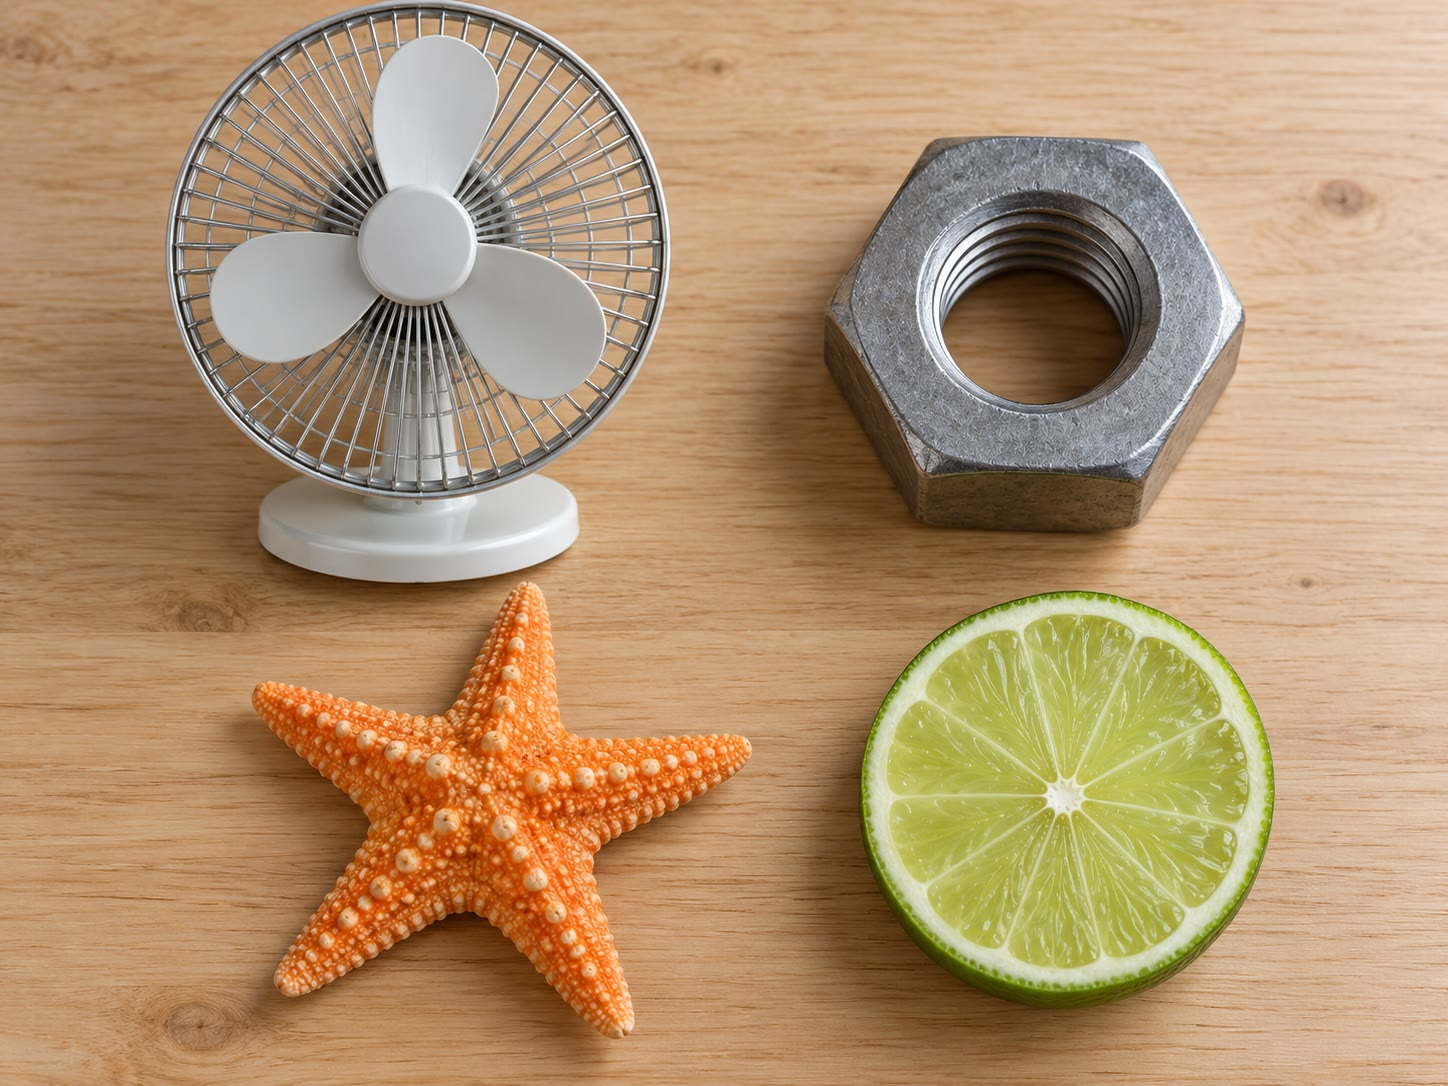
\includegraphics[width=0.48\linewidth]{images/book4/ai/b3-04-symmetric-objects.jpg}

{\small 左：威尔逊·本特利约于 1902 年拍摄的雪晶，
各具六重旋转对称性。右：日常物品，具有三重、六重
及五重旋转对称性。}
\end{omfigure}

\section{对称操作与对称元素}

\begin{definition}[对称操作，对称元素]\label{def:b3:point-groups:operation}
称\emph{对称操作}\index{对称操作}为一种运动或反射，
它使分子处于与原来不可区分的构型，
即每个原子都落在原先被同种原子占据的位置上；
称\emph{对称元素}\index{对称元素}为进行对称操作时所依据的
几何对象，即点、线或面，
或面。
\end{definition}

每个分子都有恒等操作 $E$，它什么也不做。其余的
操作分为四类。

\begin{definition}[真转轴，主轴]\label{def:b3:point-groups:rotation}
称\emph{真转轴}\index{真转轴} $C_n$ 为一条直线，
绕它作旋转 $2\pi/n$ 是一个对称操作，也记作 $C_n$；
其幂 $C_n^k$ 表示旋转 $2\pi k/n$，且 $C_n^n = E$。
取 $n$ 最大的轴为\emph{主轴}\index{主轴}，
并取为 $z$ 轴。
\end{definition}

\begin{definition}[镜面]\label{def:b3:point-groups:mirror}
称\emph{镜面}\index{镜面} $\sigma$ 为一个平面，
关于它的反射是一个对称操作，且 $\sigma^2 = E$。
若它包含主轴，则称为\emph{竖直镜面}\index{竖直镜面} $\sigma_v$；
若与主轴垂直，则称为\emph{水平镜面}\index{水平镜面}
$\sigma_h$；
若它包含主轴并平分夹角，则称为\emph{双面镜面}\index{双面镜面}
$\sigma_d$，此夹角位于与之垂直的两个
$C_2$ 轴之间。
\end{definition}

\begin{definition}[反演中心]\label{def:b3:point-groups:inversion}
称\emph{反演中心}\index{反演中心} $i$ 为一个点，
经它进行的反演 $(x, y, z) \mapsto (-x, -y, -z)$ 是
一个对称操作。
\end{definition}

\begin{definition}[象转轴]\label{def:b3:point-groups:improper}
称\emph{象转轴}\index{象转轴} $S_n$ 为一条直线，
绕它作旋转 $2\pi/n$，再接着对垂直于它的平面作反射，
所得操作是一个对称操作。$S_1 = \sigma$，$S_2 = i$。
\end{definition}

\begin{example}[四种分子的对称元素]\label{ex:b3:point-groups:elements}
\ce{H2O}：$E$，平分 H--O--H 键角的 $C_2$ 轴，以及两个
竖直面，即分子平面及与之垂直的平面。\ce{NH3}：
$E$，过 N 原子的 $C_3$ 轴（操作 $C_3$ 与 $C_3^2$），以及三个 $\sigma_v$，每个
包含一个 N--H 键。\ce{BF3}：一个 $C_3$，沿 B--F 键的三个 $C_2$，
$\sigma_h$（分子平面）、三个 $\sigma_v$，以及一个 $S_3$。\ce{CH4}：四个
沿 C--H 键的 $C_3$ 轴，平分 H--C--H 键角的三个 $C_2$，它们同时也是
$S_4$ 轴，以及六个 $\sigma_d$，每个包含两个 C--H 键
（见下图）。
\end{example}

\begin{omfigure}
\begin{tikzpicture}[font=\small]
  % H2O, side view: molecular plane xz (shaded), C2 along z
  \begin{scope}
    \fill[omDef!10] (-1.5,-1.0) -- (1.5,-1.0) -- (1.5,1.2) -- (-1.5,1.2) -- cycle;
    \fill[omThm!12, opacity=0.8] (-0.45,-1.35) -- (0.45,-0.65) -- (0.45,1.55) -- (-0.45,0.85) -- cycle;
    \draw[densely dashed, black!70] (0,-1.4) -- (0,1.7) node[above] {$C_2$};
    \node[aO] (o) at (0,0.5) {};
    \node[aH] (h1) at (-0.95,-0.25) {};
    \node[aH] (h2) at (0.95,-0.25) {};
    \begin{scope}[on background layer]
      \draw[bond] (o.center) -- (h1.center) (o.center) -- (h2.center);
    \end{scope}
    \node[omDef, anchor=north west] at (-1.5,1.2) {$\sigma_v(xz)$};
    \node[omThm, anchor=west] at (0.5,-0.85) {$\sigma_v'(yz)$};
    \node[anchor=north] at (0,-1.6) {\ce{H2O}, $C_{2v}$};
  \end{scope}
  % NH3, top view along C3
  \begin{scope}[xshift=4.0cm]
    \foreach \a in {90,210,330}{\draw[ommirror] (0,0) -- (\a:1.35); \draw[ommirror, black!40] (0,0) -- (\a+180:1.0);}
    \foreach \a in {90,210,330}{\node[aH] at (\a:0.95) {};}
    \node[aN] at (0,0) {};
    \pic at (0,0) {omthreefold};
    \node[anchor=north] at (0,-1.6) {\ce{NH3}，$C_{3v}$（从上方看）};
  \end{scope}
  % BF3, top view; sigma_h = plane of the paper (thick circle)
  \begin{scope}[xshift=8.0cm]
    \draw[ommirror] (0,0) circle (1.3);
    \foreach \a in {90,210,330}{\draw[ommirror] (\a:1.3) -- (\a+180:1.3);}
    \foreach \a in {90,210,330}{\pic[rotate=\a-90] at (\a:1.42) {omtwofold}; \pic[rotate=\a-90] at (\a+180:1.42) {omtwofold};}
    \foreach \a in {90,210,330}{\node[aF] at (\a:0.95) {};}
    \node[aX={pink!70!gray}{5.6mm}] at (0,0) {};
    \pic at (0,0) {omthreefold};
    \node[anchor=north] at (0,-1.6) {\ce{BF3}，$D_{3h}$（从上方看）};
  \end{scope}
\end{tikzpicture}

{\small 对称元素。\ce{H2O}：$C_2$ 轴（虚线）及两个竖直
镜面。\ce{NH3} 与 \ce{BF3} 沿其主轴观察（三角形
符号）：粗线为侧视所见的镜面；在 \ce{BF3} 中，粗
圆表示水平镜面（纸面所在平面），而
透镜形符号表示位于其中的三条 $C_2$ 轴。}
\end{omfigure}

\section{群}

\begin{proposition}[对称操作的乘积]\label{prop:b3:point-groups:closure}
分子的两个对称操作相继施行，结果仍是该分子的
对称操作。连同 $E$ 及各操作的逆，全体对称操作
构成一个群：乘法满足结合律，存在单位元，
每个元素都有逆元。
\end{proposition}

\begin{proof}
每个操作都使分子与自身不可区分，因此两个操作
相继施行的结果亦然。操作的乘积（空间映射的复合）
满足结合律；$E$ 是单位元；可逆的操作（即以
相反角度的旋转，或重复的反射）同样是对称操作。
\end{proof}

\begin{proposition}[公共点]\label{prop:b3:point-groups:fixed-point}
有限分子的全部对称元素都经过同一点。
\end{proposition}

\begin{proof}
每个对称操作都把每个原子映到质量相同的原子上，因此它
保持质心不变。旋转只使其
轴上的点保持不动，反射只使其平面上的点保持不动，象转轴或反演
只使一点保持不动：每个元素都包含质心。
\end{proof}

\begin{definition}[点群，点群的阶]\label{def:b3:point-groups:point-group}
分子全体对称操作构成的群称为其\emph{点群}\index{点群}，
因其有一点保持不动而得名。其对称操作的个数
称为\emph{点群的阶}\index{点群的阶}，记作
$h$。
\end{definition}

\begin{example}[水分子的群]\label{ex:b3:point-groups:c2v}
\ce{H2O} 的四个操作 $E$、$C_2$、$\sigma_v(xz)$、$\sigma_v'(yz)$ 构成一个
4 阶群。其乘法表（行上的操作在列上的操作之后
施行）如下：
\begin{center}\small
\begin{tabular}{c|cccc}
\hline
 & $E$ & $C_2$ & $\sigma_v(xz)$ & $\sigma_v'(yz)$\\ \hline
$E$ & $E$ & $C_2$ & $\sigma_v(xz)$ & $\sigma_v'(yz)$\\
$C_2$ & $C_2$ & $E$ & $\sigma_v'(yz)$ & $\sigma_v(xz)$\\
$\sigma_v(xz)$ & $\sigma_v(xz)$ & $\sigma_v'(yz)$ & $E$ & $C_2$\\
$\sigma_v'(yz)$ & $\sigma_v'(yz)$ & $\sigma_v(xz)$ & $C_2$ & $E$\\ \hline
\end{tabular}
\end{center}
例如，点 $(x, y, z)$ 经 $xz$ 平面反射后到 $(x, -y, z)$，再
以 $\pi$ 角绕 $z$ 轴旋转得 $(-x, y, z)$，与
$yz$ 中一次反射的结果相同。
\end{example}

\begin{definition}[对称操作的类，子群]\label{def:b3:point-groups:class}
两操作 $A$ 与 $B$ 属于同一
\emph{对称操作的类}\index{对称操作的类}，若 $B = X^{-1}AX$，
其中 $X$ 为群中某一操作：二者是同类操作，
在经 $X$ 移动的参照系中所见。群的子集若自身构成群，
则称为\emph{子群}\index{子群}；子群的阶整除群的阶。
\end{definition}

\begin{example}[\ce{NH3} 的类]\label{ex:b3:point-groups:classes}
在 $C_{3v}$（$h = 6$）中，三个反射构成一个类（$C_3$ 旋转
将每个平面映到另一平面），两个旋转 $C_3$ 与 $C_3^2$ 构成另一类，
$E$ 自成一类：共三个类，记为 $E$、$2C_3$、$3\sigma_v$。在
$C_{2v}$ 中，每个操作各自成一类：没有任何操作能把一个平面
变为另一个平面。
\end{example}

\begin{definition}[申夫利斯符号]\label{def:b3:point-groups:schoenflies}
点群以其\emph{申夫利斯符号}\index{申夫利斯符号}命名：
$C_n$（一个 $C_n$ 轴），$C_{nv}$（再加 $n$ 个竖直镜面），$C_{nh}$
（再加 $\sigma_h$），$D_n$（再加 $n$ 个 $C_2$ 轴，二者均与 $C_n$ 垂直），$D_{nh}$
和 $D_{nd}$（加 $\sigma_h$，或加 $n$ 个双面镜面，皆以 $D_n$ 为基础），$S_{2n}$，以及
立方群 $T_d$、$O_h$、$I_h$，分别对应四面体、八面体和
二十面体，以及 $C_s$、$C_i$、$C_1$，分别用于只有镜面、
只有反演中心或二者皆无的分子。线形分子属于
$C_{\infty v}$ 或 $D_{\infty h}$。
\end{definition}

\section{确定点群}

\begin{method}[确定分子的点群]\label{met:b3:point-groups:assign}
\begin{enumerate}
  \item 分子是否为线形？若有反演中心，则为 $D_{\infty h}$
        （\ce{CO2}、\ce{N2}）；无则为 $C_{\infty v}$（\ce{HCl}、\ce{HCN}）。
  \item 是否有多个高阶轴（$n \ge 3$）？四面体形：
        $T_d$；八面体形为 $O_h$；二十面体形为 $I_h$。
  \item 找出主轴 $C_n$（若没有，则有镜面时为 $C_s$，有
        反演中心时为 $C_i$，否则为 $C_1$）。
  \item 是否有 $n$ 个 $C_2$ 轴与 $C_n$ 垂直？若有，则群为
        $D_{nh}$（含 $\sigma_h$），否则为 $D_{nd}$（含 $n$ 个 $\sigma_d$），否则
        $D_n$。
  \item 若否：$C_{nh}$（含 $\sigma_h$）、$C_{nv}$（含 $n$ 个 $\sigma_v$）、$S_{2n}$
        （仅含 $S_{2n}$，且其与 $C_n$ 共线），否则为 $C_n$。
\end{enumerate}
\end{method}

\begin{omfigure}
\begin{tikzpicture}[font=\footnotesize, node distance=6mm and 11mm,
  q/.style={draw=black!60, fill=omDef!6, rounded corners=2pt, align=center, inner sep=3pt},
  g/.style={draw=black!60, fill=omProp!10, rounded corners=2pt, inner sep=3pt}]
  \node[q] (lin) {线形？};
  \node[g, right=of lin] (dinf) {$D_{\infty h}$ / $C_{\infty v}$（有 / 无 $i$）};
  \node[q, below=of lin] (cub) {两个或更多 $C_n$，$n \ge 3$？};
  \node[g, right=of cub] (td) {$T_d$, $O_h$, $I_h$};
  \node[q, below=of cub] (cn) {有 $C_n$ 轴？};
  \node[g, right=of cn] (low) {$C_s$、$C_i$ 或 $C_1$（否）};
  \node[q, below=of cn] (c2) {$n$ 个 $C_2 \perp C_n$？};
  \node[q, right=of c2, xshift=6mm] (dh) {$\sigma_h$？\; 否则 $n$ 个 $\sigma_d$？};
  \node[g, right=of dh] (dg) {$D_{nh}$ / $D_{nd}$ / $D_n$};
  \node[q, below=of c2] (sh) {$\sigma_h$？\; 否则 $n$ 个 $\sigma_v$？\; 否则 $S_{2n}$？};
  \node[g, right=of sh] (cg) {$C_{nh}$ / $C_{nv}$ / $S_{2n}$ / $C_n$};
  \draw[->] (lin) -- node[above] {是} (dinf);
  \draw[->] (lin) -- node[left] {否} (cub);
  \draw[->] (cub) -- node[above] {是} (td);
  \draw[->] (cub) -- node[left] {否} (cn);
  \draw[->] (cn) -- node[above] {否} (low);
  \draw[->] (cn) -- node[left] {是} (c2);
  \draw[->] (c2) -- node[above] {是} (dh);
  \draw[->] (dh) -- (dg);
  \draw[->] (c2) -- node[left] {否} (sh);
  \draw[->] (sh) -- (cg);
\end{tikzpicture}

{\small 按方法的顺序寻找点群。}
\end{omfigure}

\begin{example}[一组例子]\label{ex:b3:point-groups:gallery}
\ce{H2O}、\ce{CH2Cl2}、\ce{SO2}：$C_{2v}$。\ce{NH3}、\ce{CHCl3}：$C_{3v}$。\ce{BF3}、
\ce{PCl5}：$D_{3h}$。\ce{CH4}、\ce{CCl4}：$T_d$。\ce{SF6}：$O_h$。苯：$D_{6h}$。
乙烯：$D_{2h}$。乙烷：交叉式为 $D_{3d}$，重叠式为 $D_{3h}$。丙二烯
\ce{H2C=C=CH2}：$D_{2d}$，两个 \ce{CH2} 平面互相垂直。环己烷
在椅式构象中：$D_{3d}$。反式-\ce{N2F2}：$C_{2h}$。\ce{CHFClBr}：$C_1$。
\end{example}

\begin{omfigure}
\tdplotsetmaincoords{60}{100}
\begin{tikzpicture}[tdplot_main_coords, scale=1.6, font=\small]
  \pic[transform shape] {omcubeo={2}};
  % depth order for view 60/100 (smallest first): H(0,0,0), H(0,2,2), C, H(2,2,0), H(2,0,2)
  \draw[densely dashed, omThm, thick] (-0.4,-0.4,-0.4) -- (2.5,2.5,2.5) node[anchor=south west] {$C_3$};
  \draw[densely dashed, omDef, thick] (1,1,-0.5) -- (1,1,2.6) node[anchor=south] {$S_4$, $C_2$};
  \node[aH] (h1) at (0,0,0) {};
  \node[aH] (h4) at (0,2,2) {};
  \node[aC] (c) at (1,1,1) {};
  \node[aH] (h2) at (2,2,0) {};
  \node[aH] (h3) at (2,0,2) {};
  \begin{scope}[on background layer]
    \draw[bond] (c.center) -- (h1.center) (c.center) -- (h2.center)
                (c.center) -- (h3.center) (c.center) -- (h4.center);
  \end{scope}
\end{tikzpicture}

{\small 甲烷置于立方体中，碳原子位于中心，氢原子位于
交替的顶点上。穿过一个氢原子的体对角线是一条 $C_3$ 轴
（共四条）；穿过两个相对面心的轴是一条 $C_2$ 轴和一条
$S_4$ 轴（共三条）。该分子的点群为 $T_d$，阶为 24。}
\end{omfigure}

\section{推论：极性与手性}

\begin{theorem}[极性分子]\label{thm:b3:point-groups:polar}
分子可具有永久偶极矩，仅当其点群属于
$C_1$、$C_s$、$C_n$ 或 $C_{nv}$；此时偶极矩沿主光轴方向
（对 $C_s$，位于镜面内）。
\end{theorem}

\begin{proof}
偶极矩是分子的矢量性质，因此每个对称操作都
必须使其保持不变。绕某轴的旋转只保持沿该轴的矢量不变；
两条轴则不保持任何非零矢量；
$\sigma_h$、$i$ 或 $S_n$ 使沿该轴的任一矢量反向；$\sigma_v$
保持其所在平面内的矢量不变。因此，非零偶极矩至多要求
一条轴，不含 $\sigma_h$、$i$ 与 $S_n$，即为上述各点群。
\end{proof}

\begin{example}[极性与否]\label{ex:b3:point-groups:polar}
\ce{H2O}、\ce{NH3}、\ce{CHCl3} 和 \ce{SO2}（$C_{2v}$、$C_{3v}$）可以是极性的，
而且确实是。\ce{BF3}（$D_{3h}$）、\ce{CO2}（$D_{\infty h}$）、\ce{CH4}（$T_d$）、\ce{SF6}（$O_h$）
以及反式-\ce{N2F2}（$C_{2h}$）则不能是极性分子，无论其极性键如何。
\end{example}

\begin{theorem}[手性分子]\label{thm:b3:point-groups:chiral}
分子是手性的，当且仅当它不具有象转轴 $S_n$
（包括 $S_1 = \sigma$ 和 $S_2 = i$）。
\end{theorem}

\begin{proof}
若分子具有 $S_n$，则 $S_n = \sigma_hC_n$：分子的镜像 $\sigma_h$
等于将 $C_n^{-1}$ 作用于经 $S_n$ 作用后的分子，
亦即旋转后的分子——二者可重合，因此为非手性。反之，若
分子是非手性的，则其镜像 $\sigma M$ 可通过
一个真运动使其与 $M$ 重合（$R$ 为绕质心的旋转），于是 $R\sigma$ 为
一个对称操作。它是非真操作（改变手性，其矩阵的行列式
为 $-1$），而点群中的每个非真操作都是
某个 $S_n$（对某个 $n$，即先旋转，再在与之垂直的
平面内作反射）。因此分子具有 $S_n$。
\end{proof}

\begin{example}[无镜面的非手性分子]\label{ex:b3:point-groups:s4}
有些分子既无镜面也无反演中心，但
由于具有 $S_4$ 轴而是非手性的：典型例子为一种螺环化合物，
它由两个取代方式相同、相互成直角的环构成，其
点群为 $S_4$。仅凭寻找镜面不足以判断手性。
\end{example}

\section{表示与特征标表}

每个对称操作以线性方式移动点 $(x, y, z)$：它可以写成
一个 $3\times3$ 矩阵。

\begin{definition}[矩阵表示，特征标]\label{def:b3:point-groups:representation}
点群的\emph{矩阵表示}\index{矩阵表示} $\Gamma$ 为
每个操作 $R$ 指定一个方阵 $D(R)$，使得
$D(R_1R_2) = D(R_1)D(R_2)$：操作的乘积对应
矩阵的乘积。\emph{特征标}\index{特征标} $\chi(R)$ 是操作 $R$ 在 $\Gamma$ 中
的矩阵 $D(R)$ 的迹。
\end{definition}

\begin{example}[$C_{3v}$ 的坐标]\label{ex:b3:point-groups:xyz}
对 $C_3$（绕 $z$ 轴），$D = \begin{psmallmatrix}\cos120^\circ & -\sin120^\circ &
0\\ \sin120^\circ & \cos120^\circ & 0\\ 0 & 0 & 1\end{psmallmatrix}$，迹为
$2\cos120^\circ + 1 = 0$；对 $\sigma_v(xz)$，$D = \mathrm{diag}(1, -1, 1)$，迹为
1；对 $E$，迹为 3。该表示的特征标为 $(3, 0, 1)$，
对应于类 $(E, 2C_3, 3\sigma_v)$。每个矩阵都是分块对角的，
$2\times2$ 块对应 $(x, y)$，$1\times1$ 块对应 $z$：
该表示分裂为两个较小的表示。
\end{example}

\begin{proposition}[特征标是类函数]\label{prop:b3:point-groups:class-characters}
同一类中的操作在任何表示中具有相同的特征标。
\end{proposition}

\begin{proof}
若 $B = X^{-1}AX$，则 $D(B) = D(X)^{-1}D(A)D(X)$，而迹在
此类基变换下不变：$\mathrm{tr}(P^{-1}MP) = \mathrm{tr}(M)$。
\end{proof}

\begin{proposition}[按块约化]\label{prop:b3:point-groups:direct-sum}
若一组基可以分成若干子集，
且每个操作都把各子集映为其自身，则所有矩阵均为分块对角矩阵，
该表示是各子集所携带的较小表示之和，
其特征标等于各子集表示的特征标之和。
\end{proposition}

\begin{proof}
把各子集映为其自身的操作，
在不同子集之间没有矩阵元；分块对角矩阵的迹
等于各块的迹之和。
\end{proof}

\begin{definition}[不可约表示、特征标表、马利肯符号]\label{def:b3:point-groups:irrep}
任何基变换都无法进一步约化的表示，称为
\emph{不可约表示}\index{不可约表示}。
点群的\emph{特征标表}\index{特征标表}列出其各不可约表示的特征标，
每个不可约表示占一行，各操作类占一列，
并在表末列出按各行变换的笛卡儿函数与旋转。
各行以其\emph{马利肯符号}\index{马利肯符号}命名：
一维表示记为 $A$ 或 $B$（在主旋转下对称或反对称），
二维记为 $E$，三维记为 $T$；下标 1、2 表示在 $C_2$ 或 $\sigma_v$ 下对称或反对称，
$g$、$u$ 表示在反演下对称或反对称，
撇号表示在 $\sigma_h$ 下的性质。
\end{definition}

\begin{proposition}[特征标表的大小]\label{prop:b3:point-groups:irrep-count}
点群的不可约表示个数等于操作类的个数，
且各不可约表示维数的平方和等于群的阶：$\sum_id_i^2 = h$。
\end{proposition}
\begin{proof}[证明状态]
在\cref{ch:b3:group-theory-applied}中，由特征标的正交性证明，
而该正交性在该处被承认。
\end{proof}

% ledger: ct:C2v, ct:C3v, ct:Td
本书最常用的特征标表，
是水、氨和甲烷的特征标表：
\begin{omchartable}{C_{2v}}{cccc}{E & C_2 & \sigma_v(xz) & \sigma_v'(yz)}
A_1 & 1 & 1 & 1 & 1 & z & x^2,\ y^2,\ z^2 \\
A_2 & 1 & 1 & -1 & -1 & R_z & xy \\
B_1 & 1 & -1 & 1 & -1 & x,\ R_y & xz \\
B_2 & 1 & -1 & -1 & 1 & y,\ R_x & yz \\
\end{omchartable}
\begin{omchartable}{C_{3v}}{ccc}{E & 2C_3 & 3\sigma_v}
A_1 & 1 & 1 & 1 & z & x^2 + y^2,\ z^2 \\
A_2 & 1 & 1 & -1 & R_z & \\
E & 2 & -1 & 0 & (x, y),\ (R_x, R_y) & (x^2 - y^2, xy),\ (xz, yz) \\
\end{omchartable}
\begin{omchartable}{T_d}{ccccc}{E & 8C_3 & 3C_2 & 6S_4 & 6\sigma_d}
A_1 & 1 & 1 & 1 & 1 & 1 & & x^2 + y^2 + z^2 \\
A_2 & 1 & 1 & 1 & -1 & -1 & & \\
E & 2 & -1 & 2 & 0 & 0 & & (2z^2 - x^2 - y^2,\ x^2 - y^2) \\
T_1 & 3 & 0 & -1 & 1 & -1 & (R_x, R_y, R_z) & \\
T_2 & 3 & 0 & -1 & -1 & 1 & (x, y, z) & (xy, xz, yz) \\
\end{omchartable}

\begin{method}[读取特征标表]\label{met:b3:point-groups:matrices}
\begin{enumerate}
  \item 第一列特征标（对应 $E$）即为维数：
        该行所标记的能级或轨道的简并度。
  \item 特征标 $+1$ 表示函数在该操作下不变，
        $-1$ 表示其变号；简并行中的 0
        表示该组成员相互混合。
  \item 要确定某函数如何变换，对其逐一施加各操作，
        再与各行比较；
        右侧各列给出 $x$、$y$、$z$、旋转
        以及二次函数（$d$ 轨道的形状）的结果。
\end{enumerate}
\end{method}

\begin{example}[水中氧的轨道]\label{ex:b3:point-groups:water-orbitals}
在 $C_{2v}$ 中，氧的 $2s$ 与 $2p_z$ 轨道在每个操作下都不变，
记为 $a_1$（轨道用小写字母）。$2p_x$ 在 $C_2$ 和
$\sigma_v'(yz)$ 下变号，记为 $b_1$；$2p_y$ 记为 $b_2$。
这些是本科二年级分册中水的轨道所用的标记；
\cref{ch:b3:group-theory-applied}推导了氢组合的标记。
\end{example}

\begin{omfigure}
\begin{tikzpicture}[font=\small]
  \begin{scope}
    \pic {omstereo={1.2}};
    \draw[ommirror] (-1.2,0) -- (1.2,0);
    \draw[ommirror] (0,-1.2) -- (0,1.2);
    \pic at (0,0) {omtwofold};
    \foreach \x/\y in {0.55/0.45,-0.55/0.45,0.55/-0.45,-0.55/-0.45}{\pic at (\x,\y) {omup};}
    \node[anchor=north] at (0,-1.35) {$C_{2v}$};
  \end{scope}
  \begin{scope}[xshift=4cm]
    \pic {omstereo={1.2}};
    \foreach \a in {90,210,330}{\draw[ommirror] (\a:1.2) -- (\a+180:1.2);}
    \pic at (0,0) {omthreefold};
    \foreach \a in {70,110,190,230,310,350}{\pic at (\a:0.75) {omup};}
    \node[anchor=north] at (0,-1.35) {$C_{3v}$};
  \end{scope}
  \begin{scope}[xshift=8cm]
    \pic {omstereo={1.2}};
    \draw[ommirror] (0,0) circle (1.2);
    \foreach \a in {90,210,330}{\draw[ommirror] (\a:1.2) -- (\a+180:1.2);}
    \pic at (0,0) {omthreefold};
    \foreach \a in {70,110,190,230,310,350}{\pic at (\a:0.75) {omup}; \pic at (\a:0.75) {omdown};}
    \node[anchor=north] at (0,-1.35) {$D_{3h}$};
  \end{scope}
\end{tikzpicture}

{\small 立体投影图。赤道面以上的一般点（圆点）经该群各操作，
映为图中所示的全部点；位于赤道面以下的点用叉号标记。
粗线与圆为镜面。$C_{2v}$：4 个点；$C_{3v}$：6 个；
$D_{3h}$：12 个（上方 6 个，下方 6 个，重叠）：
点的个数即为群的阶。}
\end{omfigure}

\begin{history}[申夫利斯与晶体的对称性]
阿图尔·申夫利斯是一位数学家，他于 1891 年对晶体的 230 个空间
群作了分类；他所命名的 32 个晶体学点群至今仍
沿用他所定的符号。化学家于 20 世纪 30 年代开始采用这套记号，
那时群论开始应用于分子光谱。
\end{history}

\begin{inthelab}[用分子模型套件研究对称性]
要找出陌生分子的对称元素，最快的办法是用分子模型套件把它搭起来，
拿在手中转动，寻找这样的轴：绕其转动不到一圈，分子便与原来重合，
以及能把分子切成互为镜像两半的平面。
计算程序也能在一定容差范围内给出
优化结构的点群。
\end{inthelab}

\section{练习}

\begin{exercise}[$\star$]\label{exo:b3:point-groups:1}
列出下列分子的对称元素并给出其点群：乙烯、\ce{XeF4}、
\ce{PCl5}、1,3,5-三氯苯。
\end{exercise}

\begin{exercise}[$\star$]\label{exo:b3:point-groups:2}
给出交叉式和重叠式乙烷以及环己烷的
椅式构象的点群。
\end{exercise}

\begin{exercise}[$\star$]\label{exo:b3:point-groups:3}
下列分子中哪些可能是极性分子：\ce{SO3}、\ce{SO2}、\ce{PCl3}、\ce{XeF4}、\ce{CH2Cl2}、
顺式和反式-1,2-二氯乙烯？
\end{exercise}

\begin{exercise}[$\star$]\label{exo:b3:point-groups:4}
写出 $3\times3$ 矩阵，分别表示 $C_2(z)$、$i$ 和 $\sigma_h$
作用于 $(x, y, z)$ 的情形，并求出它们的特征标。
\end{exercise}

\begin{exercise}[$\star\star$]\label{exo:b3:point-groups:5}
作出 $C_{2h}$ 的乘法表，所用操作为 $E$、$C_2$、$i$、
$\sigma_h$。每个操作是否都自成一类？
\end{exercise}

\begin{exercise}[$\star\star$]\label{exo:b3:point-groups:6}
在 $C_{3v}$ 中，通过跟踪一个点，计算 $\sigma_v(1)\,C_3$ 与 $C_3\,\sigma_v(1)$。
二者是否相等？这说明该群具有什么性质？
\end{exercise}

\begin{exercise}[$\star\star$]\label{exo:b3:point-groups:7}
证明：使两环之间扭转角介于 0 与 90\textdegree\ 之间的联苯，
属于 $D_2$，并由此判断其手性。
\end{exercise}

\begin{exercise}[$\star\star$]\label{exo:b3:point-groups:8}
利用 $C_{2v}$ 特征标表，求水分子中氧原子 $3d$ 轨道的
符号（取二次函数作为其形状）。
\end{exercise}

\begin{exercise}[$\star\star$]\label{exo:b3:point-groups:9}
在 $T_d$ 特征标表上验证 $\sum_id_i^2 = h$，并验证行 $A_1$ 与 $T_2$
在各列按其类的大小加权时彼此正交。
\end{exercise}

\begin{exercise}[$\star\star\star$]\label{exo:b3:point-groups:10}
证明：两镜面夹角为 $\theta$ 时，二者乘积是绕其交线的
转角为 $2\theta$ 的旋转。由此推出：具有两个竖直镜面、夹角为
60\textdegree\ 的分子具有 $C_3$ 轴。
\end{exercise}

\begin{exercise}[$\star\star\star$]\label{exo:b3:point-groups:11}
丙二烯 \ce{H2C=C=CH2} 的两个 \ce{CH2} 基团位于相互垂直的平面内。求出其全部对称元素，
证明其点群为 $D_{2d}$，并说明为何
1,3-二氯丙二烯 \ce{ClHC=C=CHCl} 具有手性。
\end{exercise}

\begin{exercise}[$\star\star\star$]\label{exo:b3:point-groups:12}
从 \ce{SF6}（$O_h$）出发，依次得到 \ce{SF5Cl}、反式-\ce{SF4Cl2} 和
顺式-\ce{SF4Cl2}，分别给出各点群，并证明每个点群都是
$O_h$ 的子群。其中哪些可能是极性分子？
\end{exercise}

\section{问题：取代甲烷}

\begin{problem}[{周末问题——甲烷的 24 个对称操作，
其氯代衍生物的点群，依据定理判断极性与手性，
以及同分异构体的计数}]
\label{pb:b3:point-groups:1}
% ledger: ct:Td
甲烷画在一个边长为 2、以原点为中心的立方体内，氢原子位于
顶点 $(1,1,1)$、$(1,-1,-1)$、$(-1,1,-1)$ 和 $(-1,-1,1)$ 上。

\medskip\noindent\textbf{第一部分——甲烷的群。}
\begin{enumerate}
  \item 求出四条 $C_3$ 轴，并计算它们给出的旋转操作个数。
  \item 求出三条 $C_2$ 轴，并验证每条也是 $S_4$ 轴；
        计算 $S_4$ 操作的个数。
  \item 求出六个镜面，以及每个镜面所含的 C--H 键。
  \item 加上 $E$：该群的阶是多少？
  \item 验证不存在反演中心。（$(-1,-1,-1)$ 是否为氢原子的
        位置？）
  \item 将这些操作按 $T_d$ 特征标表的五个类进行分组。
\end{enumerate}

\medskip\noindent\textbf{第二部分——氯代甲烷。}
\begin{enumerate}[resume]
  \item 给出 \ce{CH3Cl} 的点群及其阶。
  \item \ce{CH2Cl2} 的同样问题。
  \item \ce{CHCl3} 和 \ce{CCl4} 的同样问题。
  \item \ce{CH2FCl} 和 \ce{CHFClBr} 的同样问题。
  \item 验证每个点群都是 $T_d$ 的子群，且其阶整除 24。
  \item \ce{CH3Cl} 的哪些氢原子可由其操作互换？
\end{enumerate}

\medskip\noindent\textbf{第三部分——极性与手性。}
\begin{enumerate}[resume]
  \item 六种分子中哪些可能为极性分子？给出每个
        偶极矩的方向。
  \item 哪些是手性分子？
  \item 对于手性分子，有多少种立体异构体？
  \item 为什么 \ce{CH2FCl} 虽然其碳原子以四个键分别与
        三种不同的原子相连，却是非手性的？
  \item 具有四个不同取代基的甲烷衍生物，是否可能
        为极性分子却不具手性？
  \item $T_d$ 的哪一个表示是由碳原子的三个
        $2p$ 轨道所张成的？
\end{enumerate}

\medskip\noindent\textbf{第四部分——同分异构体计数。}
\begin{enumerate}[resume]
  \item 证明：甲烷中任意两个氢原子，都可经 $T_d$ 的某一操作
        被移到任意另外两个氢原子的位置上。\ce{CH2Cl2} 有多少种同分异构体？
  \item \ce{CH2FCl} 有多少种同分异构体？计入对映异构体后，\ce{CHFClBr} 有多少种？
  \item 苯（$D_{6h}$）有多少种二氯苯？给出它们的
        点群。
  \item 有多少种三氯苯？给出它们的点群。
  \item 若将“甲烷”设想为平面正方形（$D_{4h}$），
        \ce{CH2Cl2} 将有多少种同分异构体？这一论证在历史上证明了什么？
  \item 验证 $T_d$ 的阶等于其各不可约表示维数的
        平方和，并叙述这一结论。
\end{enumerate}
\end{problem}
